\chapter{Difference-in-Differences}
\label{ch-did}

This chapter is based on
Ref.\cite{book-mixtape}.


The Difference-in-Differences (DID)
method was first used by John Snow
in an 1854 report that
argued that 
cholera in London
was being transmitted 
by sewage polluted water
rather than, as others
at the time believed, by air (in fetid vapors
called miasmas).
In general, one can
apply DID to discover 
causal effects in historical data.
By {\bf historical data} (aka a {\bf natural
experiment}. See Ref.\cite{wiki-nat-exp})
we mean data that is collected long
after the treatment (rather than during it)
 and is thus
not  subject to 
active intervention
by the experimenter. 

This chapter assumes that the
reader has read Chapter \ref{ch-pot-out}
on Potential Outcomes (PO).
The DID method
applies the basic single-time
PO theory described in Chapter \ref{ch-pot-out},
to 2
well separated times
in which
different conditions prevail.



\section{John Snow, DID  
and a cholera
transmission pathway}


\begin{figure}[h!]
\centering
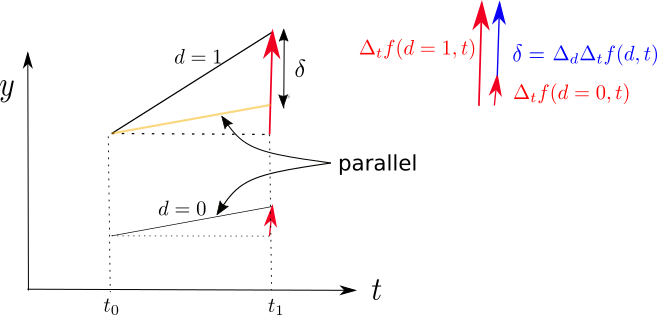
\includegraphics[width=5in]
{did/dif-dif.png}
\caption{Pictorial representation of
 Difference-in-differences (DID) as a difference
of two differences (i.e., 
a difference of two slopes).} 
\label{fig-dif-dif}
\end{figure}

Let

$d\in \bool$

$t\in \{t_0, t_1\}$, $t_0< t_1$

$y=f(d,t)\in \RR$.

Define

\beq
\Delta_t f(d,t)= f(d, t_1)-f(d, t_0)
\;,
\eeq

\beq
\Delta_d f(d, t)= f(1, t)-f(0, t)
\;,
\eeq

\beq
DID=\delta=\Delta_d\Delta_t f(d,t)
\;.
\eeq
DID is illustrated in
 Fig.\ref{fig-dif-dif}. 


A {\bf time series} 
is  any function of time
for which the domain is a discrete set of times.




\begin{figure}[h!]
\centering
\includegraphics[width=4in]{did/did-3-prod}
\caption{$DID=\delta$ expressed as 
difference of slopes or 
difference of vectors.} 
\label{fig-did-3-prod}
\end{figure}

Note that,
as shown Fig.\ref{fig-did-3-prod},
$DID=\delta$ can also be expressed
as a difference of 2 slopes
times $\Delta t = t_1-t_0$.
Let
$\hat{y}$ be a unit 
in the $y$ direction.
$\delta$ can also be expressed
as the dot product of a difference of 2 vectors
dotted with $\hat{y}$.


\begin{table}[h!]
\centering
{\renewcommand{\arraystretch}{1.4}
\begin{tabular}{|c|c|c|}
\hline 
\rowcolor[HTML]{ECF4FF} 
 & $t=t_0 $ (1849) & $t=t_1$ (1854) \\ 
\hline
$d=1 $ (town 1)\cellcolor[HTML]{ECF4FF}
&85 deaths, polluted DW&19 deaths, unpolluted DW\\
\hline 
$d=0 $ (town 0)\cellcolor[HTML]{ECF4FF} 
&135 deaths, polluted DW& 147 deaths, polluted DW\\ 
\end{tabular}
}
\caption{A condensation of the data
collected by 
John Snow in 1854,
to test the hypothesis
that cholera in London was being spread by
polluted drinking water (DW).}
\label{tab-john-snow}
\end{table}

A condensation of the
data collected by John Snow in 1854
is given in Table \ref{tab-john-snow}.
From that data, we find that

\beq
\delta= \Delta_d\Delta_t f(d,t)=(19-85)-(147-135)=
-66-12=-78
\eeq



\section{PO analysis}
In this section,
we show how
to analyze the
DID method
using the formalism of PO theory.

We will speak of a treatment 
outcome
$\rvy^\s_{t, g^\s}
(c^\s, x^\s)$
for individual $\s$
that depends, not 
just on the treatment dose 
$c^\s\in \bool$
and the confounder state $x^\s$,
but also
on a group parameter (i.e., which population
or town)
$g^\s\in \bool$
and on a time parameter $t\in\{t_0, t_1\}$ 
(note $t$ is independent of $\s$).
Actually,
we will assume $g^\s=c^\s$,
so we will just speak of
$\rvy^\s_t(c^\s, x^\s)$
with no explicit $g^\s$
dependence. As usual for PO theory,
we will consider
expected values of $y^\s_t$:


\beq
E_{\s| d, x}[y^\s_t(c)]=
 E_{\rvy_t(c)| d, x}[\rvy_t(c)]=
\caly_{c| d, x}(t)
\eeq

To calculate these
expected values, we need a ``model"
with probability 
distributions.
In this case,
the needed model and probability
distributions are
provided by the
bnets depicted in Fig.\ref{fig-did-G_t-+}.
The TPMs,
printed in blue,
for the 
 bnet
$G_{t, +}$
in Fig.\ref{fig-did-G_t-+},
are as follows.
Note
that the
TPMs for the bnet $G_{t, +}$
are defined in 
terms
of the TPMs for the bnet $G_t$.


\begin{figure}[h!]
$$
\begin{array}{ccccc}
\xymatrix{
&\rvx\ar[dl]\ar[dr]
\\
\rvd\ar[rr]&&\rvy_t
}
&&
\xymatrix{
&&\rvx\ar[d]\ar[ddll]
\\
&&[\rvy_t(0), \rvy_t(1)]
\ar[d]
\\
\rvd\ar[rr]
&&\rvy_t
}
\\
\\
G_t&&G_{t, +}
\end{array}
$$
\caption{$t\in \{t_0, t_1\}$.
Bnet 
$G_{t,+}$
is obtained 
by adding
two new nodes
$\rvy_t(0)$
and $\rvy_t(1)$ to bnet $G_t$.}
\label{fig-did-G_t-+}
\end{figure}

\beq\color{blue}
P(x)=P_{\rvx}(x)
\eeq

\beq\color{blue}
P(d|x)= 
P_{\rvd|\rvx}(d|x)
\eeq
 
\beq\color{blue}
P(y_t| y_t(0), y_t(1),d)=
\indi(y_t=y_t(d))
\eeq

\beq\color{blue}
P(y_t(c)|x)=
P(y_t(c)|d,x)=\text{given}
\eeq

\begin{figure}[h!]
\centering
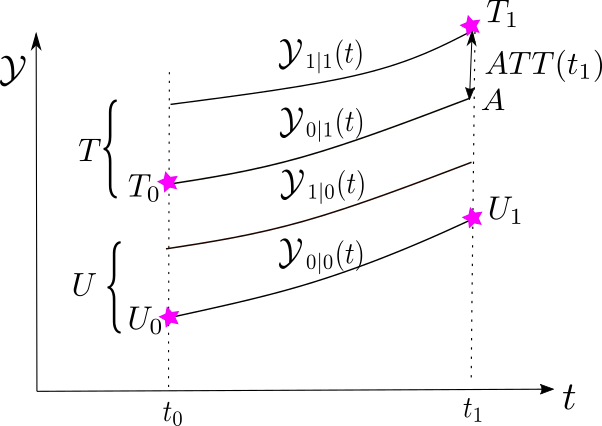
\includegraphics[width=4in]
{did/dif-dif-bc.png}
\caption{
Four different time-dependent
expected 
values $\caly_{c| d}(t)$ of $y^\s_t$
for bnet $G_{t, +}$
The 4 magenta  stars
represents the 4 DID measurements.
} 
\label{fig-dif-dif-bc}
\end{figure}



We define the function $c(t)$ for $t=t_0, t_1$ by

\beq
c(t)
=
\left\{
\begin{array}{ll}
0&\text{if $t=t_0$}
\\
 d&\text{if $t=t_1$}
\end{array}
\right.
\eeq
Now we claim that the DID 
$\delta$ calculated in the 
previous section for
John Snow's data,
can be expressed in PO formalism as follows:

\beq
\delta=
\Delta_ d\Delta_t
\caly_{c(t)| d}(t)
\;.
\eeq
Fig.\ref{fig-dif-dif-bc}
depicts the
four functions
$\caly_{c| d}(t)$
for $t$ in the interval  $[t_0, t_1]$
and for $c, d\in \bool$.
The $\caly$ coordinates
of the four magenta stars in 
Fig.\ref{fig-dif-dif-bc} can 
be calculated using bnet $G_t$.

Define
the {\bf parallel trends} (PT)
by 

\beq
PT=\Delta_ d\Delta_t\caly_{0| d}(t)
\;.
\eeq
We will say the 
{\bf parallel trends assumption (PTA)}
holds if $PT=0$.

Next we prove that
the DID $\delta$ equals
the sum of an ATT\footnote{ATT stands for 
the average treatment effect
of the treated. ATT is defined 
in Chapter \ref{ch-pot-out}}
and PT.

\begin{align}
\delta&=
\Delta_ d\Delta_t  
\caly_{c(t)| d}(t)
\\
&=
\left[
\Delta_t \caly_{c(t)|1}(t)
-\Delta_t \caly_{c(t)|0}(t)
\right]
\\
&=
\caly_{1|1}(t_1)-\caly_{0|1}(t_0)
-\{
\caly_{0|0}(t_1)-\caly_{0|0}(t_0)
\}
\\
&=
\caly_{1|1}(t_1)-\caly_{0|1}(t_0)
-\{
\caly_{0|0}(t_1)-\caly_{0|0}(t_0)
\}
+\underbrace{
\{
\caly_{0|1}(t_1)-
\caly_{0|1}(t_1)
\}}_{\text{ zero }}
\\
&=
\underbrace{
\caly_{1|1}(t_1) - \caly_{0|1}(t_1)}
_{ATT(t_1)}
-\caly_{0|1}(t_0)
-\{
\caly_{0|0}(t_1)-\caly_{0|0}(t_0)
\}
 + \caly_{0|1}(t_1)
\\
&=
ATT(t_1)
-\Delta_t \caly_{0|0}(t)
+\Delta_t \caly_{0|1}(t)
\\
&=
ATT(t_1)
+
\underbrace{\Delta_ d\Delta_t\caly_{0| d}(t)}_
{\text{ zero if PTA holds}}
\end{align}





\section{Linear Regression}
In this
section,
we show how to apply
linear regression (LR)
to the PO analysis of DID.


As before, let
$y^\s_t(c^\s)$ be the treatment outcome
for individual $\s$,
who receives
a treatment dose
$c^\s$
at times $t\in\{t_0, t_1\}$.
$y^\s_t(c^\s)$
can be fitted as follows.
Here $\eps^\s$
is the residual
for individual $\s$,
and $b_0, m_0, b_1, m_1\in \RR$
are the fit parameters.

\beq
y^\s_t = [b_0 + m_0 (t-t_0)](1-c^\s)
+  [b_1 + m_1 (t-t_0)]c^\s
+ \eps^\s
\;.
\label{eq-did-lr}
\eeq  
Note that Eq.(\ref{eq-did-lr})
 yields a straight line
in the $y^\s_t-t$ plane
for $c^\s=0$,
and another 
straight line for $c^\s=1$.
We are
using the
standard symbols
$b$ to denote
the y-intercept, and $m$ 
to denote the slope
of a straight line.

Taking the expected value
of Eq.(\ref{eq-did-lr}), we get

\beq
\caly_{c| d}(t) = 
[b_0 + m_0 (t-t_0)](1-c)
+  [b_1 + m_1 (t-t_0)]c
\;.
\eeq  
If $\Delta  t = t_1-t_0$, then

\beq
\caly_{ d| d}(t_1) = 
[b_0 + m_0 \Delta t](1- d)
+  [b_1 + m_1 \Delta t] d
\;,
\eeq
and

\beq
\caly_{0| d}(t_0) = b_0
\;.
\eeq
 Thus,   

\beqa
\delta&=&\Delta_ d\Delta_t 
\caly_{c(t)| d}(t)
\\
&=&
\Delta_ d[\caly_{ d| d}(t_1)-\caly_{0| d}(t_0)]
\\
&=&
(m_1-m_0)\Delta t
\;.
\eeqa



\begin{figure}[h!]
\centering
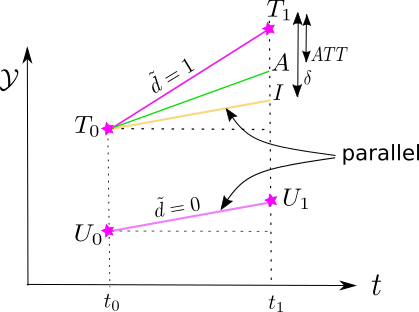
\includegraphics[width=3.5in]
{did/parallel-trends.png}
\caption{We use
Linear Regression
to fit a straight line
between points $U_0$
and $U_1$,
and between points
$T_0$ and $T_1$.
(U=untreated, T=treated, subscript refers
to times $t_0, t_1$).
$U_0, T_0, U_1, T_1$ are the measurement points.
Point
$I$ is an image of point $U_1$.
} 
\label{fig-parallel-trends}
\end{figure}

\begin{table}[h!]
\centering
{\renewcommand{\arraystretch}{1.2}
\begin{tabular}{|c|c|c|}
\hline 
\rowcolor[HTML]{ECF4FF} 
 & $t=t_0$ & $t=t_1$ \\ 
\hline
$ d=1$ \cellcolor[HTML]{ECF4FF}& 
$\caly(T_0)=\caly_{0|1}(t_0)$ & 
$\caly(T_1)=\caly_{1|1}(t_1)$ \\ 
\hline 
$ d=0$\cellcolor[HTML]{ECF4FF} & 
$\caly(U_0)=\caly_{0|0}(t_0)$ & 
$\caly(U_1)=\caly_{0|0}(t_1)$ \\ 
\hline 
\end{tabular}
}
\caption{
$\caly$ coordinates
of points
$U_0, T_0, U_1, T_1$
in Figs.\ref{fig-dif-dif-bc}
 and \ref{fig-parallel-trends}.
}
\label{tab-did-points}
\end{table}



Figs.\ref{fig-dif-dif-bc} and
\ref{fig-parallel-trends}
define
points $U_0, T_0, U_1, T_1, I, A$.
The $\caly$
coordinates of points 
$U_0, T_0, U_1, T_1$ are 
given by
Table \ref{tab-did-points}.
The $\caly$
coordinates of points $A,I$
are given by Eqs.\ref{eq-c-i-pts}.

\begin{subequations}
\label{eq-c-i-pts}
\beq
\caly(A)= \caly_{0|1}(t_1)
\eeq

\beq
\caly(I)=\caly(U_1) + 
[\caly(T_0)-\caly(U_0)]
\eeq
\end{subequations}

We can express $ATT$
and the $\delta$ for DID 
in terms of 
the $\caly$
of the points
$U_0, T_0, U_1, T_1, I, A$. Indeed,

\beqa
\delta&=&\caly(T_1)-\caly(I)
\\
&=&
\caly(T_1)-
\caly(U_1) -
[\caly(T_0)-\caly(U_0)]
\eeqa

\beq
ATT = \caly(T_1)-\caly(A)
\eeq
Hence, 

\beq
\delta=ATT\iff \caly(I)=\caly(A) \iff 
\text{PTA holds}
\eeq